\section{Protocol description}

Each command is termintad by a newline character, and each value in a command is seperated by a whitespace.

Overview of packets:
\begin{table}[h!]
	\centering
	\label{Protocol:overview}
	\begin{tabular}{lllll}
		\# & Description 		& Commando    		& Direction             & Example     		\\
		0  & Handshake   		& RollingRoad 		& PSoC $\rightarrow$ PC & 0 RollingRoad 	\\
		1  & Unit description 	& <int> <str> <str> & PSoC $\rightarrow$ PC & 1 0 Time Seconds 	\\
		2  & Stop        		&            		& PC $\rightarrow$ PSoC	& 2        			\\
		3  & Information 		& <double> ... <double>	& PSoC $\rightarrow$ PC & 3 2 3 	    	\\
		4  & Torque control 	& <int>    			& PC $\rightarrow$ PSoC & 4    				\\
	\end{tabular}
	\caption{Overview for commands sent between PSoC og PC}
\end{table}

In figure \ref{fig:TimingDiagram}, the flow of communication can be seen. Starting with the handshake initiated by the PC, followed by the PSoC repeating.

After the handshake, the PSoC transmits all type and units this source can collect.

\fixme{Flip handshake direction}
\begin{figure}
\centering
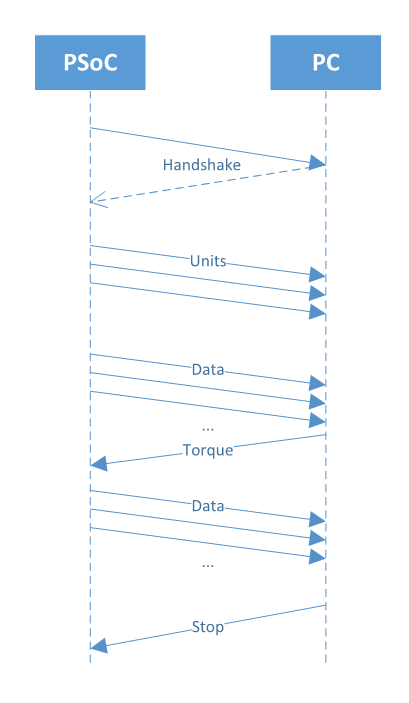
\includegraphics[width=0.5\linewidth]{Protocol/TimingDiagram}
\caption{}
\label{fig:TimingDiagram}
\end{figure}

\fixme{Create in-depth description of each}